\documentclass[a4paper,11pt]{article}
\usepackage[margin=2.5cm]{geometry}
\usepackage{amsmath}
\usepackage{amssymb}
\usepackage{graphicx}
\usepackage{caption}
\usepackage{natbib}

\date{Draft \today}
\title{Towards a Universal Veering Profile for Turbulent Ekman Flow at arbitrary Reynolds number \\
  \normalsize LES and DNS of Turbulent Ekman Flow \\}

\begin{document} 

\maketitle

\begin{abstract}
  An analytical formulation for the profiles of stream- and span-wise velocity in turbulent Ekman flow
  is developed based on asymptotic theory as well as data from direct numerical simulation and large-eddy simulation.
  %
  The profile of the stream-wise component follows the classical viscous, logarithmic and wake scaling.
  %
  The span-wise component poses a conceptual challenge to the channel-flow analogy
  in the context of asymptotic mixing, and it exhibits a mixed scaling in the surface layer, but follows
  outer scaling for most of the outer layer.
  %
  In both profiles, the wake region can be described by smooth error-function transition from a logarithmic layer
  to the constant outer velocity.
  
\end{abstract}
%
%%%%%%%%%%%%%%%%%%%%%%%%%%%%%%%%%%%%%%%%%%%%%%%%%%%%%%%%%%%%%%%%%%%%%%%%%%%%%%%%
%
\section{Introduction}

The exact veering of the wind away from its geostrophic direction is due to direct and indirect (due to turbulence) frictional effects,
and it plays a role for various practical problems: 
%
It sets the amount of cross-isobaric volume flow and is thus a key factor in the life-cycle of large-scale synoptic systems. This mechanism is commonly
referred to as 'Ekman pumping' referring to the perturbation of the geostrophic equilibrium that causes the veering as it was first described
and solved for analytically by \cite{Ekman:1905tl}.
%
On the mesoscale, shear in the surface layer is known to be crucial for the initiation and sustainment of strong convective events (REFERENCE?).
% 
And locally, directional sheer of the wind in the upper part of the surface layer may cause a yaw for large wind power generation devices (REFERENCE?).
%
%%%%%%%%%%%%%%%%%%%%%%%%%%%%%%%%%%%%%%%%%%%%%%%%%%%%%%%%%%%%%%%%%%%%%%%%%%%%%%%%
%
\section{Formulation}
%
\paragraph{Physical Problem.} We consider incompressible, turbulent Ekman flow, i.e. the turbulent flow over a flat rotating plate, as
a physical model for the truly neutral atmospheric boundary layer (ABL).
%
That is, the f-plane approximation is used confining effects of rotation to the horizontal components of
velocity and neglecting dynamical effects due to latitudinal changes of the rate of rotation. 
%
%%PAR
%
\paragraph{Notation.} The dimensional velocity vector of the numerical simulations is $\underline{U} = (U_1,U_2,U_3) = (U,V,W)$ over the coordinate system
$Oxyz$, where an approximate alignment with the surface shear stress is achieved.
%
For analysis of the results, we use two coordinate systems that are
(i)  exactly aligned with the surface shear stress and labelled by an upper index $\alpha$ as in $\underline{U}^\alpha$ for the velocity vector, and
(ii) the coordinate system aligned with the free-atmosphere geostrophic wind labelled by an upper index $G$ as in $\underline{U}^G$.
%
We denote by $u_\star$ the modulus surface friction velocity and let $Z_\star=1/u_\star$ for brevity. 

\section{Towards a Universal Velocity Profile for the Turbulent Ekman Layer}
\subsection{Drag-Law} 
The drag law for Ekman flow, including prediction of surface veering, has received considerable attention in the past.
\begin{itemize}
\item \cite{Rossby:1935wa} first approach;
\item \cite{Tennekes:1973jh, Blackadar:1968ew} asymptotic similarity;
\item \cite{Spalart:1989p2436, Spalart:2008p2432, Spalart:2009p2466} seminal LES studies in search for a universal log-law;
\item \cite{Ansorge:2014hf, Ansorge:2019di} re-evaluation of the constants with geophysical focus;
\item \cite{Hogstrom:1988wg, Hgstrm:1996kt} (re-)consideration of observational data.
  %

\end{itemize}
\begin{figure}
  \centerline{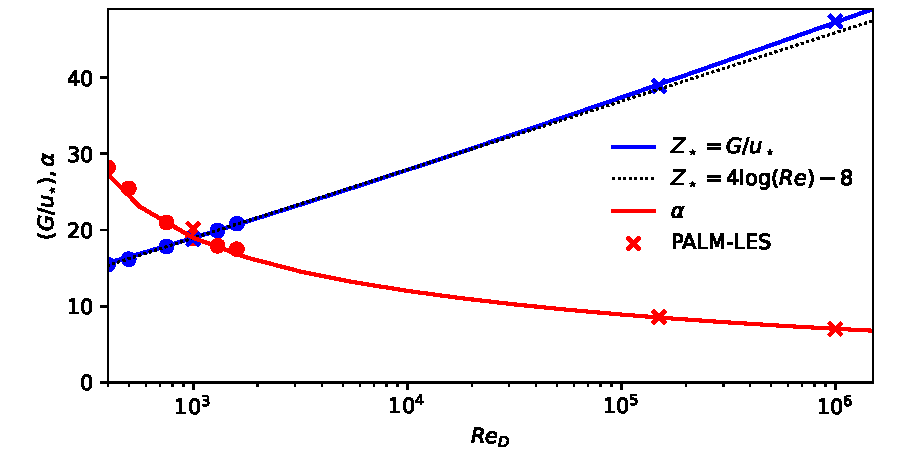
\includegraphics[width=0.7\textwidth]{ustar_alpha.pdf}}
  \caption{Variation of $Z_\star$ and surface veering with Reynolds number according to
    the theory by Spalart et al. (1989) and as estimated from DNS data}
  \label{fig:drag_law}
\end{figure} 
%
Attempts were also undertaken to obtain profiles of the wind speed: 
\cite{Gryning:2007dy} present an extension of the wind-speed profile beyond the surface layer using a neutral referece profile
and a stability correction;
\cite{Kelly:2010ev}, based on a probabilistic representation of stratification, develop a model for the long-term mean windspeed
in the atmospheric boundary layer and compare this with observation at different sites; 
\cite{Kelly:2016bs} demonstrate the effect of such improved model for wind-energy applications.
%
These investigations merely focus on the wind speed and thus do not regard the actual vector, i.e. the veering of
the wind with height is not described and there is little knowledge on the profile of the span-wise velocity component
and the precise shape of the hodograph in the limit of a truly neutral Ekman boundary layer.
%
While this is indeed an academic problem, the Ekman boundary layer often serves as limit for stratified boundary layers
and thus not only needs to be understood but also well-described as reference for higher-order approaches that take into
account possible effects of stratification, roughness or other physical complications of the geophysical system.
%
\subsection{Stream-wise Velocity} 
For the stream-wise velocity profile (that in non-rotating flows due to the geometry is always aligned with the surface shear stress),
well-established theories exist for various regimes according to their distance from the wall and the relative role of
viscosity, turbulence and interaction with the outer region of the flow with the logarithmic law for the mean velocity as a central anchor point:
\begin{subequations}
  \begin{itemize}
  \item In immediate vicinity to the surface, local turbulent mixing cannot occur for the no-slip/no-penetration boundary condition,
    and the mean velocity is described by a viscous profile of the form
    \begin{equation}
      (U,W)^{\alpha+}  = (z^+,0)  
    \end{equation}
    where the direction of 
    in absence of roughness elements are marginal linear regime / viscous sub-layer \cite{Foken:2002gv,Foken:1978bc} 
  \item buffer layer transition from linear regime to log-law  
  \item log-layer (K\'arm\'an, Prandtl, Jimenez, Marusic)
  \item outer log-layer () 
  \item wake region
  \item outer region 
  \end{itemize}
\end{subequations} 
%
\begin{figure}
  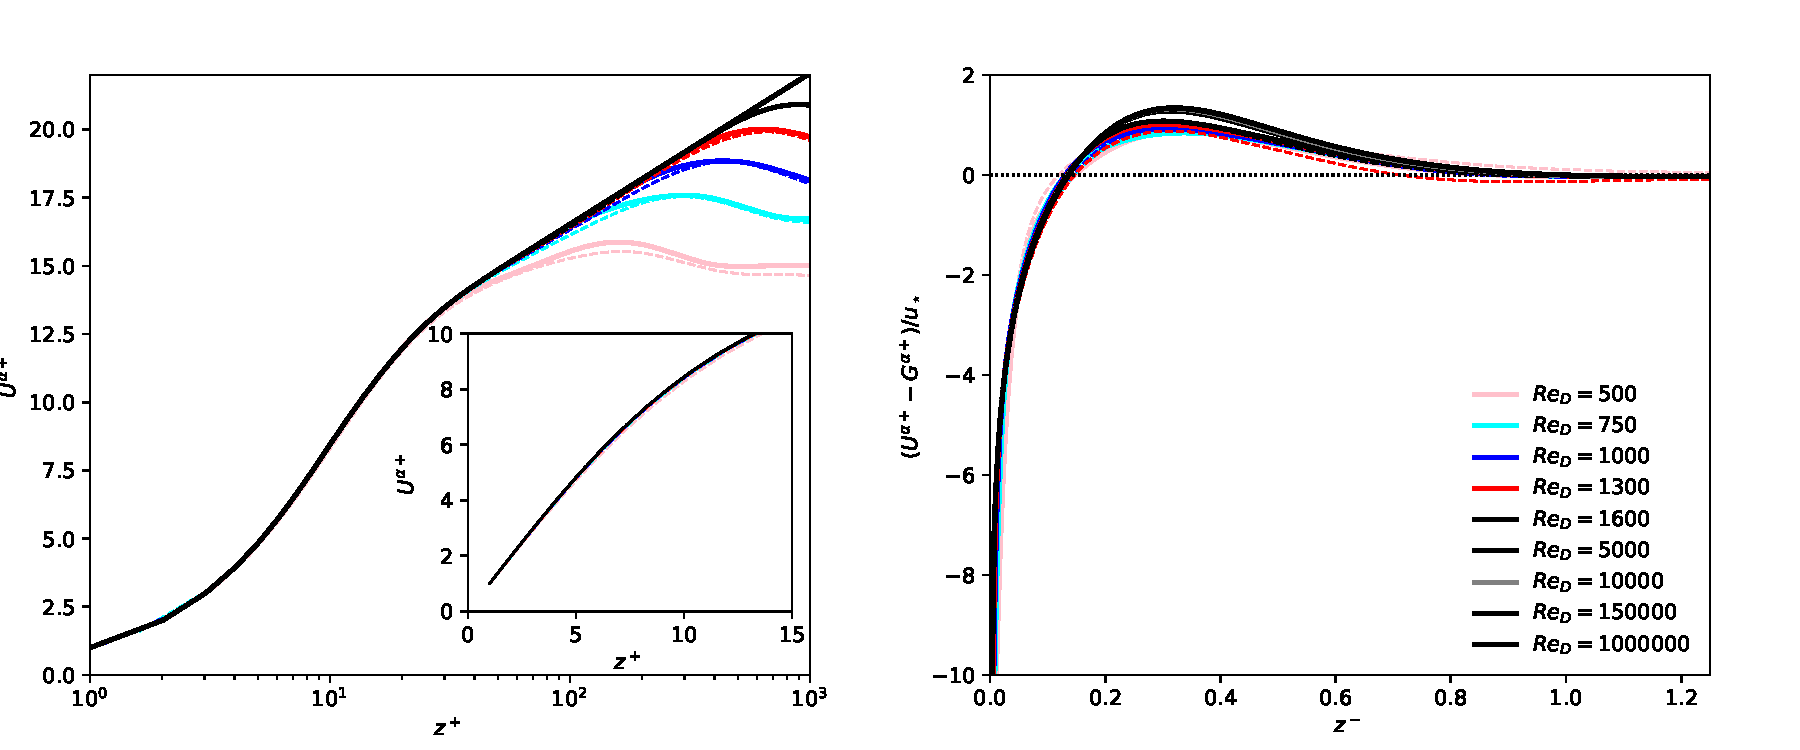
\includegraphics[width=\textwidth]{u_profile.pdf}
  \caption{Shear-aligned profiles of velocity components $U^{\alpha+}$ in inner (left) and outer (right) units.} 
\end{figure} 

Existing theories applied to the boundary layer:
\begin{itemize}
\item \cite{Etling:2002kx, Emeis:2018vq}  (Sec. 21.10; Eq. 21.48) -- ad-hoc matching at Prandtl-layer height; requires $\alpha$ 
\item \cite{Emeis:2007cy} (Sec. 3; Eq. 3.1-3.19) -- 1D profile; considering constant (?) veering 
\item \cite{Gryning:2007dy} (Mean wind profiles)
\end{itemize}

For non-rotating, non-external flows theoretical considerations by Townsend (cite to attached-eddy hypothesis)
have recently been confirmed from both wind-tunnel  experiments and numerical simulation \cite{Ng:2011bk,Marusic:2013hf}
implying physical models for the second moments (Reynolds stresses) of the flow.
%
\subsection{Span-wise velocity} 
%
The background rotation and associated veering of the surface wind implies a non-zero profile for the span-wise velocity that
challenges the conventional assumptions related to the so-called channel-flow analogy:
%
While the universal profiles in vicinity of the wall implies that the profile be zero or at least small with respect to the stream-wise
component, the veering requires a value of $V_{top}=U_G\sin\alpha$ in the free stream (and thus also at the top of the boundary layer if we assume
that substantial velocity gradients are confined to the turbulent part of the flow). 
%
This is commonly shown in terms of velocity hodographs aligned with the outer, geostrophic flow (cf. Fig.~\ref{fig:hodograph}) and normalized by
the geostrophic wind. 
%
Thus, the drag-law already implies three important properties of these hodographs,
(i) the boundary conditions at the surface,
(ii) the boundary condition at the top, and
(iii) the inclination of the hodograph at the origin by the surface veering:
\begin{subequations} 
\begin{eqnarray} 
 \underline{U}^{G}(z=0) &=& 0,\\ 
 \underline{U}^{G}(z\mapsto\infty) &=& \underline{G}^G = \left(\begin{array}{c}1\\0\end{array}\right) \\
   \left.\frac{\partial V^G}{\partial U^G}\right|_{z=0} &=& \sin\alpha
\end{eqnarray} 
\end{subequations} 
%
Outer scaling of the velocity profile further implies that the velocity deficity of the spanwise component $V^\alpha-G^\alpha$
be a universal function of the outer height $z^-$, i.e.  
\begin{eqnarray}
  V^\alpha-G^\alpha = f^\alpha_V(z^-).  
\end{eqnarray}
%
Interpreting the shear-aligned spanwise velocity deficit $f_{V}^{\alpha}(z^-)$ as 
a signature of outer rotation may lead one to conclude that this universal function
is appropriate down to the surface--irrespective of the Reynolds number.
%
This cannot be the case for the variation of $f_{V}^{\alpha}(z^-)$ across the boundary layer (i.e. between $0<z^-<1$)
must fulfill the drag law and boundary conditions;
at the same time, the weak dependence of $\alpha$ and $u_\star$ on $Re$ implies this range depends on $Re$.
%
%%%PAR
%
\paragraph{Outer Layer.} In the outer region of the flow (for $z^-\mapsto 1$), $f_V(z^-)$, should govern the
spanwise velocity profile which indeed is supported by our DNS data (Fig.\ref{fig:outer_w}):
%
The deficit is close to zero for $z^-\gtrsim 1$, and can be approximated by a logarithmic profile in the
range $0.15\lesssim z^- \lesssim 0.4$.
%
The slope of this profile is best fit by $\kappa_V=0.836 (1 + 150 / Re_D) \kappa$, where the correction term for low Reynolds number
may be omitted for $Re_D \gg 1000$.
%
Based on Fig.~\ref{fig:outer_w}, we pick the offset as
a constant fraction (0.906) of $V^\alpha_G=Z_\star \sin\alpha$, i.e
\begin{subequations} 
\begin{align}
  V_\text{log}(z^-)  = \frac{1}{\kappa_V} \log\left(\frac{z^-}{0.4}\right) + 0.906V_G^{\alpha}. 
\end{align} 
%
%%%PAR
% 
The eventually converged simulations at intermediate $Re_D$ (where the DNS could be run over several inertial periods)
exhibit a super-geostrophic maximum (positiv velocity deficit) in the span-wise component.
%
This maximum is not present or less pronounced for the simulations at higher $Re$ where closer analysis reveals that the
velocity profiles in the outer layer are still subject to a small though finite adaptation process on the inertial time
scales $2\pi/f$ due to the relatively short time span for which these cases could be simulated.
%
While there is no physical model for this wake region that leads to an analytical velocity profile formulation in the span-wise direction,
an error-function transition from the outer logarithmic law to the boundary condition provides a reasonable fit:
%
\begin{align}
  V_\text{outer}(z^-) = (1-w_V)V_\text{log}(z^-) + w_V V_G^\alpha
\end{align} 
with
\begin{align} 
w_V = \frac{\mathrm{erf}\left[\xi_\text{outer} \log(z/z_\text{ref})\right]  + 1}{2}
\end{align}
where $\xi_\text{outer}$ is a transition scale that defines the width of the wake region and $z_\text{ref}$ defines the height.
Based on the DNS data, we choose $\xi_\text{outer}=2$ and let $z_\text{ref}$ such that $V_\text{log}(z_\text{ref}) = 0.98V_G^\alpha$.
There is, however, a degree of ambiguity in the exact choice of these parameters due to the imperfect convergence of the
DNS data to the statistical equilibrium.
%
\end{subequations} 
%
%%% PAR
%
\paragraph{Inner Layer.} It is important to note that the logarithmic layer observed here for the spanwise velocity does not
conincide with the log-region of the streamwise velocity but is rather a 'continuation' through the outer layer.
%
This is consistent with the recent finding of a second log-region in the outer region of Ekman flow
(... et al. (incl. Sullivan), JAS 2019).
%
Below this region, the gradients in span-wise velocity are rather small and the span-wise velocity
monotonically approaches its surface boundary condition $V(z=0)=0$.
%
While the stream-wise velocity follows a universal inner scaling that has acquired its universal, $Re$-independent shape for $Re_D> \mathcal{O}\left(10^3\right)$, the span-wise component that defines how the velocity vector veers when the surface is approached,
does not collapse in inner units, and there is, most importantly no sign of convergence even at the highest Reynolds numbers for
which simulations where carried out.
%
Even though the simplest assumption $V=0$ is reasonable for the lower part of the surface surface layer ($z^-<10^{-3}$), it does
not appropriately capture the profile in the rest of the surface layer:

First, $V=0$  implies a discontinuity in the velocity profile at $z^-=0.1$, where the outer scaling found above 
yields a finite value at geophysical $Re$, i.e. there is non-zero veering in the upper part of the
surface layer--as is well-known also from field observation. 
%
Second, the layer around $z^-=0.1$ is crucial to obtain the characteristic and well-established shape of the hodographs as the layer
where $V$ sets in marks the 'maximum' of $V^-$ vs. $U^-$.
%
This illustrates that the higher-order (in terms of the channel-flow analogy where $V=0$) correction follows a mixed scaling when the surface is approached which has been demonstrated for higher-order terms in other types of flow \citep{Mellado:2016hv}. 
%
\par
%
The scale for the magnitude of the span-wise velocity component is $u_\star\sin\alpha$. 
%
Based on our DNS data, we suggest that the Reynolds number scaling of this velocity-magnitude scale is captured
by $Re_\tau^{-1/2}$ which is indeed known from the generalization of higher-order statistics, such as turbulent fluxes
in the inner layer \citep{Marusic:2013hf} that also follow a mixed scaling in the inner layer.
%
We then parameterize the spanwise velocity at 10 wall units as anchor point in the inner layer:
\begin{subequations}
\begin{align}
  V_{10}\equiv V(z^+=10)=750 \frac{u_\star\sin\alpha}{\sqrt{Re_\tau}}.
\end{align} 
%
This leaves us with three fixed points of the velocity profile in the inner layer, namely
(i) the boundary condition $V_0=0$,
(ii) $V_{10}$ at $z^+=10$, and 
(iii) the lower end of the logarithmic profile at $z^-=0.1$ where the latter two are semi-empirically estimated
from DNS data. 
%
In absence of well-established scaling considerations for the span-wise velocity, the choice of profile fits joining
these three points is indeed arbitrary, but we can resort to the DNS data for an empirical approach and find
that a square-root profile fits $V(z^+)$ in the surface layer.
%
A linear profile for $V$ is employed in the viscous sub-layer.
%
Based on the physical extent of the viscous sub-layer in Ekman flow around five wall units \citep{Foken:2002gv, Ansorge:2019di},
we choose $z^+=5$ to transition from one to the other and note that $V$ is already very small at this height.
%
The span-wise velocity profile in the surface layer is then estimated as 
\begin{align}
  \left.V(z^+)\right|_{\text{inner}} = \left\{\begin{array}{c c l}
  a_1 z^+&;& z^+ \le 5\\ 
  b_1+b_2 \sqrt{z^+}&;& 5<z^+<Re_\tau/10 
  \label{eqn:w_profile_inner}
  \end{array} \right, 
\end{align}
with $b_1$ and $b_2$ estimated such that
\begin{eqnarray}
  \begin{array}{r c l} 
    \left.V(z^+=10)\right|_\text{inner}&=&V_{10}\\
    \left.V(z^+=Re_\tau/10)\right|_\text{inner}&=&V_{\text{outer}}(0.1)\\
  \end{array}
  \Rightarrow \left\{ \begin{array}{l}
    b_2=\dfrac{V_\text{outer}(0.1) - V_{10}}{\sqrt{Re_\tau/10}-\sqrt{10}}  \\[1.5em]
    b_1= V_{10} - \sqrt{10}b_2
  \end{array}\right. 
\end{eqnarray}
We then estimate $\alpha$ from the matching condition at $z^+=5$, i.e.
\begin{align}
  5a = b_1+\sqrt{5}b_2 \Rightarrow a = \frac15 \left[V_{10} + (\sqrt{5}- \sqrt{10})\left(\frac{V_\text{outer}-V_{10}}{\sqrt{Re_\tau/10}-\sqrt{10}}\right) \right].
  \label{eqn:alpha_coefficient} 
\end{align}
%
%%%PAR
%
\paragraph{Matching region.} While the profile composed of $V_\text{inner}(z^+\le 0.1 Re_\tau)$, $V_\text{outer}(z^->0.1)$ is continuous,
it is not smooth at $z^-=0.1$, i.e. at the transition from power-law ($V\propto \sqrt{z^+}$) to logarithmic scaling.
%
To alleviate this issue, we use a second-order polynomial for transition from the inner to the outer layer in the range
$z_\text{low}<z<z_\text{up}$ such that
\begin{align} 
  V_\text{trans}(z^-) &=& V_\text{inner}(z^+_\text{low}) + \Delta V \left(a z_{arg} + b (z_{arg})^2\right)
\end{align}
with $\Delta V &=& V_\text{outer}(z^-_\text{up})-V_\text{inner}(z^+_\text{low})$
and  $z_{arg} = (z - z_\text{low})/(z_\text{up}-z_\text{low})$.
It is  $a+b=1$ for $V_\text{trans}(z^-_\text{up}) = V_\text{outer}(z^-_\text{up})$, and we constrain $a$ by
\begin{align}
  \left.\frac{\partial V_\text{trans}}{\partial z^-}\right|_{z=z_\text{low}} = \left.\frac{\partial V_\text{inner}}{\partial z^-}\right|_{z=z_\text{low}},
\end{align}
where we find that $z^-_\text{low}=0.06$ and $z^-_\text{up}=0.13$ yield satisfactory agreement with DNS data. 
 
%
\begin{figure}
  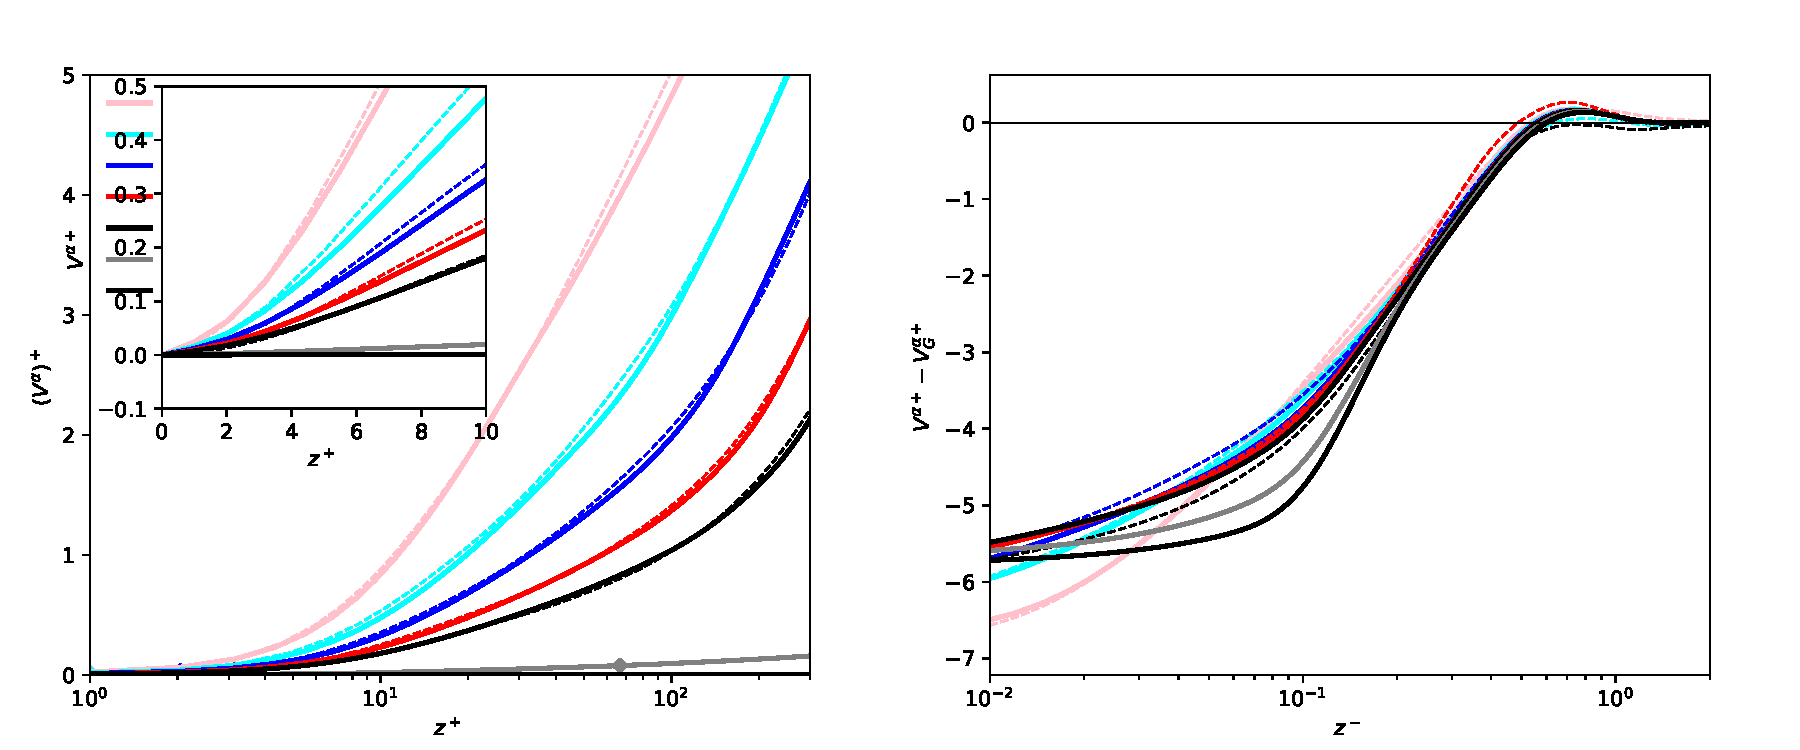
\includegraphics[width=1.0\textwidth]{w_profile.pdf}
  \caption{Profiles of shear-aligned span-wise velocity $(W^\alpha)^+$ versus inner and outer height.
  Dashed lines show DNS data, thick, opaque lines are from the semi-emprical theory developed above. }
  \label{fig:outer_w} 
\end{figure}
\end{subequations}



\begin{figure}
  \phantom{AAA}\textbf{(a)\hspace{0.3\textwidth}(b)\hspace{0.3\textwidth}(c)}\\
  \includegraphics[width=\textwidth]{ekman_profiles_data.pdf}
  \caption{ \textbf{(a)} Velocity deficity, \textbf{(b)} velocity profile in shear-aligned hodographs and \textbf{(c)} hodograph in geostrophy-aligned coordinates.
    Thick, solid lines show theory, dashed lines data from DNS. }
  \label{fig:hodograph} 
\end{figure} 

\section{Comparison with other theories}

\textbf{Compare} to Emeis (2002) and Gryning (2007); highlight explicit knowledge on veering-profile $\rightarrow$ directional sheer;
%
\par%%%%%%%%%%%%%%%%%%%%%%%%%%%%%%%%%%%%%%%%%%%%%%%%%%%%%%%%%%%%%%%%%%%%%%%%%%%%%%%%
%
Implications for \textbf{K-theory} (we now can consider that shear and stress are not necessarily perfectly aligned).
$\rightarrow$ can we do something to infer a K-profile from these theoretical considerations? 
%
\begin{figure}
  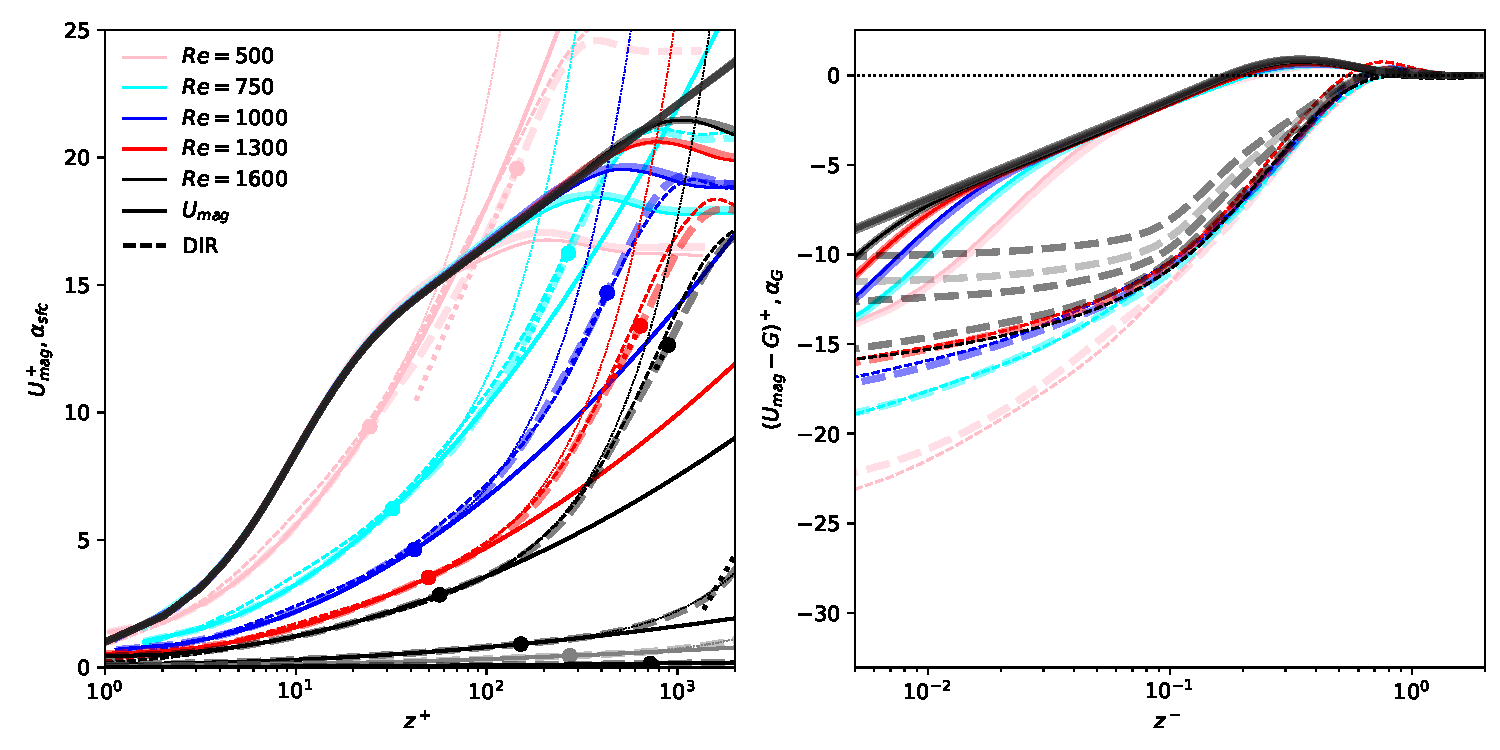
\includegraphics[width=\textwidth]{mag_dir.pdf} 
  \caption{Total velocity and veering (in degrees) vs inner and outer height.
    Dashed lines show DNS data, thick lines are from semi-empirical theory.} 
\end{figure} 
%
\section{Conclusions}
%
Applications:
\begin{itemize}
\item reference-shear for neutral profile approaches(systematic!) $\rightarrow$ wind engineering! 
\item initial condition for LES/DNS to eliminate/minimize inertial oscillation in Benchmark simulations
\item 
\bibliographystyle{plainnat}
\bibliography{ansorge.bib}
\end{document} 
